\Chapter{Új adatok előállítása, generatív modellek}
A generatív modellek alatt olyan gépi-tanulásos architektúrákat értünk, amelyek célja, hogy új adatot állítson elő. A létrejött adatnak hasonlítania kell a tanítómintához, vagyis a generált minták eloszlásának közelítenie kell a valós adatok eloszlását. Az ilyen modelleknek meg kell tanulnia a tanítóminta jellegzetességeit és azt is, hogy ezen jellegeket a belső reprezentációjából hogyan tudná értelmezhető formában előállítani. A generatív modellek esetében ha a modell a tanítóminta képeit generálná csupán vissza pixel-pontosan, úgy a modell elveszti célját és egyfajta ovefitting-nek tekinthetnénk a jelenséget.

Az Autoencoder egy olyan statisztikai elveken alapuló architektúra, amelynek célja, hogy a tanítóhalmaz jellegzetességeit feltérképezze és olyan formába kódolja a tulajdonságokat, hogy azokból az eredeti adat visszaállítható legyen. Az architektúra lényegében egy nehezen kezelhető sűrűségfüggvényt definiál, egy látens taggal, így ebben az esetben nem lehet közvetlenül optimalizálni, nem úgy mint például a pixelRNN/pixelCNN generatív modellek esetében \cite{oord2016conditional}, hanem az úgynevezett \textit{evidence lower bound} (ELBO) mértékegységre kell optimalizálni\cite{oord2017neural}. Az architektúra két komponense az Encoder, amely előállítja a jellegvektorokat a bemenet alapján és a Decoder, amely a jellegvektorokból visszaállítja az adatot. Tehát ebben az esetben a cél az, hogy egy olyan reprezentációt készítsünk a tanítómintáról, amely alapján az teljes mértékben visszaállítható legyen. Egyfajta tömörítési folyamatnak is felfogható az encoder működése. Egy módosított változattal az encoder által létrehozandó látens tér olyan formában áll elő, amelyből véletlenszerűen is vehetünk mintákat és dekódolva teljesen új adat áll elő. Ezt a módszert Vector Quantised-Variational AutoEncoder-nek nevezték el, amely alkalmazható generatív modellként \cite{oord2017neural}.
Ha az autoencoder-t képek generálására kívánjuk felhasználni, úgy a helyreállított képeken egyfajta homályosságot figyelhetünk meg, amely a dekódolás során jelentkező információvesztésből adódik.

A Generative Adverserial Network (GAN) \cite{goodfellow2014generative}, egy olyan generatív modell, amely nem a megszokott statisztikai alapokon optimalizál, mint például az Autoencoder vagy pixelRNN modellek, hanem játékelméleti megközelítést alkalmaz, így a modell tanítása is merőben másképp zajlik.
A tanulás során két neurális hálózat versenyzik egymással: egy generátor, amelynek az a szerepe, hogy a tanítómintákhoz hasonló adatot generáljon a bemeneti zajból és egy diszkriminátor, amely egy bináris osztályozó, amely a generátor által generált adatot vizsgálja és eldönti, hogy az valódi vagy hamis.
A tanítás során ezen két háló versenyzik egymással, együtt fejlődve. Az autoencoderhez képest a GAN-al generált képeken már nem figyelhető meg a homályosság, élesebb és fotórealisztikusabb képek generálása a fejlettebb GAN architektúrákkal megoldható.

A generátor bemenete egy zajvektor, amely általában Gauss- vagy egyenletes eloszlásból állítunk elő. A zajnak a terét az irodalom látens térnek is nevezi, hiszen a tanítás során a modell megtanulja, hogy ezen többdimenziós tér egyes pontjaira milyen kimenetet generáljon. Vagyis ezzel lényegében kitölti a rendelkezésre álló tér tartományait a megtanult jellegzetességekkel. A betanított generátorral, optimális esetben, ezen tér bármely pontját mintavételezve a tanítóhalmazhoz hasonló adatokat generálhatunk.

\begin{figure}[h]
\centering
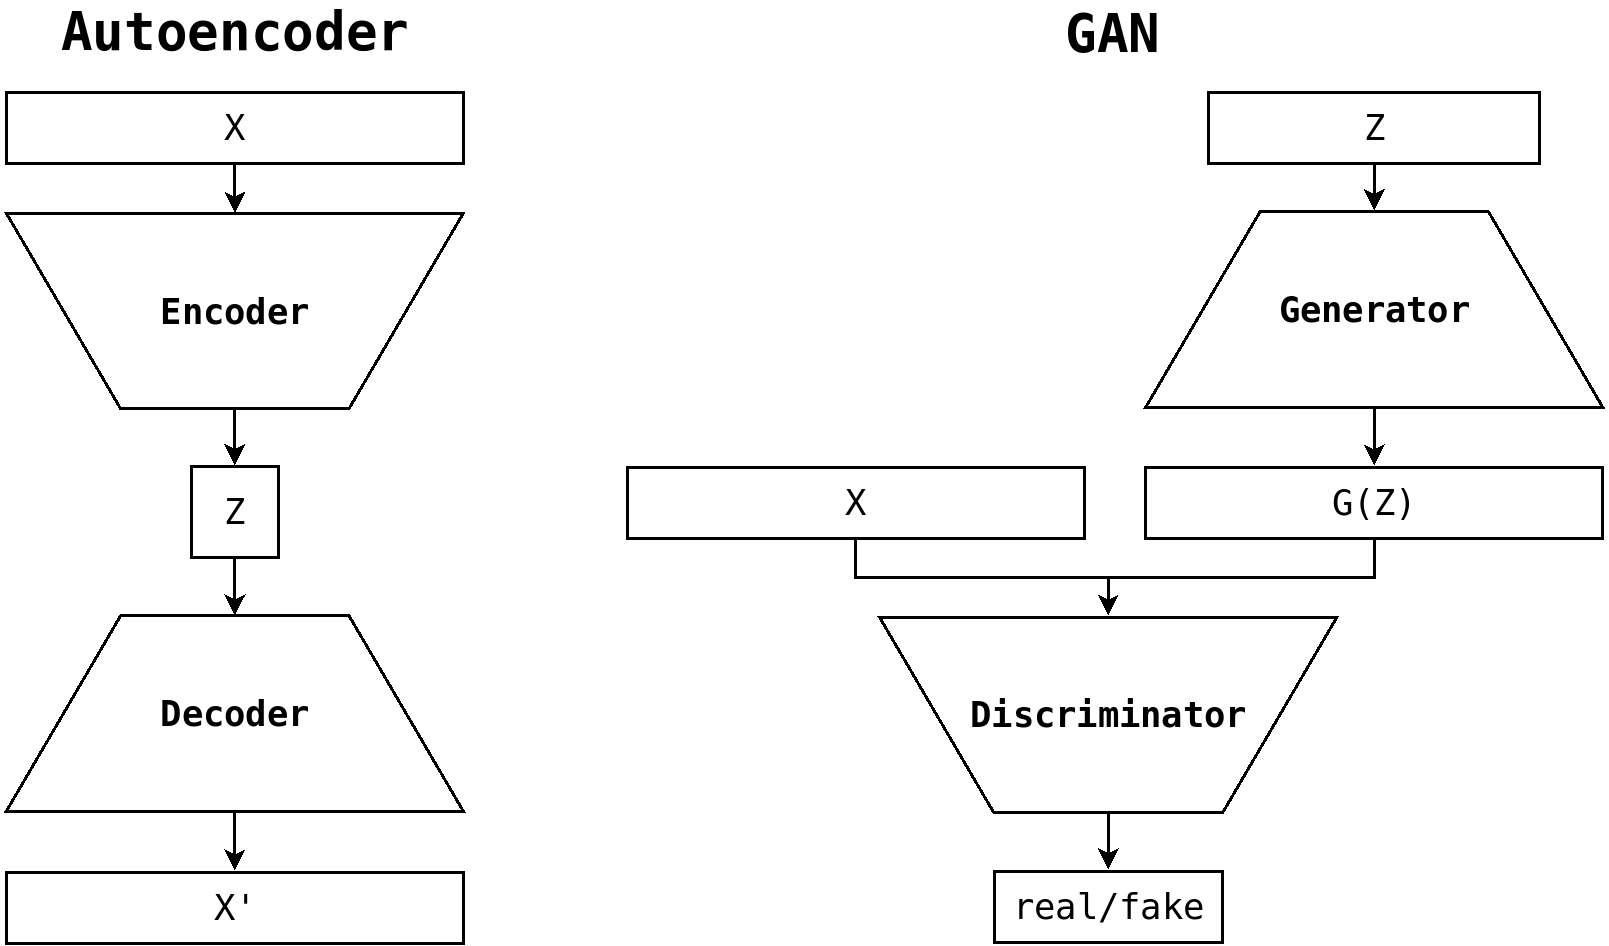
\includegraphics[width=12cm]{images/AEvsGAN.png}
\caption{Az Autoencoder és a GAN}
\label{fig:aevsgan}
\end{figure}

\Section{GAN modell tanítása}

Ha a legegyszerűbb esetet vizsgáljuk és csak a képek rendezetlen halmazára tanítjuk a modellt, mindenféle kiegészítő információ és annotáció nélkül, akkor a tanítás a következőképpen zajlik.
A továbbiakban a következő jelöléseket használom: legyen $D$ a diszkriminátor, $G$ pedig a generátor.

\SubSection{Hibafüggvények}

A $G$ és $D$ hibájának számolása a bináris kereszt-entrópián alapszik.
A bináris kereszt-entrópia hibafüggvény a következőképpen írható fel:
$$L(\hat y, y) = y . \log \hat y + (1-y). \log (1 - \hat y)$$
Ahol $\hat y$ a predikció, $y$ pedig a valós címke.

\begin{python}
cross_entropy = keras.losses.BinaryCrossentropy(from_logits=True)
\end{python}

A Kerasban található implementáció egy segédfüggvényt ad vissza, amelyet különféle paraméterekkel inicializálhatunk. A \texttt{from\_logits=True} paraméter esetén a keresztentrópia számolásnál nem szükséges a diszkriminátor modellnek tartalmaznia az utolsó sigmoid aktivációs függvényét, ami így egy úgynevezett \textit{Logits} kimenettel fog rendelkezni. A számolás során a kimeneti értékekre alkalmazódik ebben az esetben a sigmoid függvény egy fajtája. A gradiensek számolása így egyszerűbb lesz a modell számára a backpropagation során (Tényleg?)

\SubSection{Diszkriminátor hibafüggvénye}

A $G$ generátor egy $z \in \mathbb{R}^n, n \geq 1$ bemeneti zajvektor alapján előállít egy generált adatot $G(z)$.
A $D$ diszkriminátor egy bináris osztályozó, amelynek feladata, hogy az $x$ és $G(z)$ bemeneteit osztályozza.

$D(x)$ esetén 1, $D(G(z))$ esetén pedig 0 címkét várunk.

A hibafüggvény számolása két lépésben történik a kétféle bemenet miatt:

$D(x)$-re nézve a kereszt-entrópia a következő:
$$L(D(x), 1) = 1.\ln D(x) + (1 - 1).\ln(1 - D(x))$$
$$L(D(x), 1) = \ln D(x)$$
Vagyis jelen esetben $D$-nek a $\ln(D(x))$-et kell maximalizálnia.

$D(G(z))$-re nézve a kereszt-entrópia a következő:
$$L(D(G(z)), 0) = 0.\ln D(G(z)) + (1 - 0).\ln(1 - D(G(z)))$$
$$L(D(G(z)), 0) = \ln(1- D(G(z)))$$
Vagyis a $\ln(1 - D(G(z)))$-t kell maximalizálnia.

Egyetlen mintára a hibafüggvény a következőképpen néz ki:
$$\max V(D) = \ln D(x) + \ln(1 - D(G(z))$$

Batch-ra nézve:
$$\max V(D) = \mathbb{E}_{x \sim P(x)} \left[\ln D(x) \right] + \mathbb{E}_{z \sim P(z)} \left[\ln(1 - D(G(z))) \right]$$

Ahol a $P(x)$ a valószínűségi eloszlása a tanítóhalmaznak, $P(z)$ a valószínűségi eloszlása a $z$ zajvektornak. (látens tér).

\begin{python}
def discriminator_loss(real_output, fake_output):
    real_loss = cross_entropy(tf.ones_like(real_output), real_output)
    fake_loss = cross_entropy(tf.zeros_like(fake_output), fake_output)
    
    total_loss = real_loss + fake_loss
    return total_loss
\end{python}


\SubSection{Generátor hibafüggvénye}

A $G$ generátor feladata az, hogy megtévessze a $D$ diszkriminátort azáltal, hogy a tanítóhalmazhoz hasonló adatokat generáljon.
Vagyis a $G$ érdeke az, hogy a $D(G(z))$ 1-es címkét kapjon 0 helyett.

Tehát a bináris keresztentrópia egy mintára:
$$L(D(G(z)), 0) = \ln(1 - D(G(z))$$
$D$ minimalizálni kívánja a $D(G(z))$-t, míg a $G$ maximalizálni szándékozik azt.

A $G$ a tanítás során sosem fog valódi adatot látni, de a teljesség kedvéért a hibafüggvénye a következőképpen írható fel (Csak a második kifejezést minimalizálja valójában):
$$\min V(G) = \mathbb{E}_{x \sim P(x)} \left[\ln D(x) \right] + \mathbb{E}_{z \sim P(z)} \left[\ln(1 - D(G(z))) \right]$$

\begin{python}
def generator_loss(fake_output):
    return cross_entropy(tf.ones_like(fake_output), fake_output)
\end{python}

Vagyis a GAN hálózat tanítása során $D$ és $G$ egy minimax játékot játszanak a $V(G, D)$ értékfüggvénnyel.
$$\min_{G}\max_{D}V(D, G) =  \mathbb{E}_{x \sim P(x)} \left[\ln D(x) \right] + \mathbb{E}_{z \sim P(z)} \left[\ln(1 - D(G(z))) \right]$$

\SubSection{Optimalizáló módszer}
A GAN modell súlyait a sztochasztikus gradiens algoritmussal szokás frissíteni.

A Generátort és a Diszkriminátort a hibafüggvények alapján kiszámolt gradiensek alapján külön-külön kell tanítani. Különféle szerzők különböző optimalizáló módszerek használatát javasolják, az Adam \cite{kingma2014adam} és az RMSProp a két legnépszerűbb módszer.

%TODO: Optimalizáló módszerek bemtatása!

\begin{python}
generator_optimizer = keras.optimizers.Adam(1e-4)
discriminator_optimizer = keras.optimizers.Adam(1e-4)
\end{python}


\SubSection{Tanítási lépés}
A GAN esetében a hálózat paraméterei közé tartozik a mini-batch elemszáma is. Mini-batch alatt a tanítóhalmaz egy bizonyos elemszámú mintát tartalmazó szeletét értjük. A mini-batch-ok alkalmazása azért lényeges, hogy egy tanítási lépés során a modell ne lássa a teljes tanítóhalmazt. A hálózat tanításához általában sok mintára van szükségünk, így az egy darabban való tanítás igen nehézkes és számításigényes lenne. De nem csupán ez jelenti a fő veszélyt, Ha egy lépésben láthatná a diszkriminátor az összes képet, akkor túlságosan is megnőne a teljesítménye és a generátornak esélye sem lenne felzárkózni. A mini-batch-okon való tanítás tehát elengedhetetlen része a tanítási folyamatnak és a megfelelő ütemű tanulás biztosításának.
A fellelhető irodalomban a mini-batch-ot néhány esetben röviden batch-nak nevezik. Viszont a batch egyes irodalmakban a teljes dataset-et jelöli, így az egyértelműség kedvéért minden esetben kiírom a mini-batch-ot.

%% GAN 2014 cikkből

A GAN hálózat egy tanítási lépése a következő lépésekből áll \cite{goodfellow2014generative}:

Legyen $m$ a minibatch elemszáma $m \in \mathbb{N}$
\begin{enumerate}
\item Hozzunk létre $m$ darab zajmintát $(z_1, \ldots, z_m)$ gauss eloszlásból $P_g(z)$.
\item A tanítóhalmazból emeljük ki a soron következő $m$ darab tanítómintát (képet), és ezt jelöljük $(x_1, \ldots, x_m)$-el $P_{\text{data}}(x)$
\item Frissítsük a $D$ diszkriminátort a sztochasztikus gradiens emelkedésével (?? tükörfordítás)
$$ \nabla \theta_d \frac{1}{m} \sum_{i=1}^{m} \left[\log D(x_i) + \log(1 - D(G(z_i))) \right]$$
\item  Frissítsük a $G$ generátort a sztochasztikus gradiens lejtésével (?? tükörfordítás)
$$ \nabla \theta_d \frac{1}{m} \sum_{i=1}^{m} \log(1 - D(G(z_i)))$$
\end{enumerate}

A GAN részeit tehát külön-külön tanítjuk, hiszen különböző neurális hálókról van szó. Az eredeti cikkben is javaslatot tesznek arra, hogy a $D$-t esetleg több lépésben is lehetne tanítani, majd a $G$-t egyetlen lépésben frissíteni.
Különböző tanítási stratégiákban ez is egy szabad paraméter lehet. Számomra megfelelő volt az 1:1-es tanítási lépés alkalmazása is. Viszont több cikkben is vizsgálják ezt, mint lehetséges beállítást.
A tanítás hossza természetesen függ az adathalmaztól és annak méretétől, az alkalmazott mini-batch mérettől, a modellben található paraméterektől és az optimalizáló eljárástól.

A TensorFlow-ban és Kerasban történő tanítási lépés megvalósítása a következő kódrészletben figyelhető meg. A \texttt{@tf.function} annotáció segítségével jelezhetjük a TensorFlow backendnek, hogy az annotációval ellátott függvényt fordítsa le (PONTOSÍTÁS). Az annotáció használata a kritikus, nagy erőforrás-igényű és ismétlődő számolásoknál a futásidőt csökkentheti. Az függvény első meghívásánál felállítja a függőségi vagy hívási gráfot is, ezzel is csökkentve a futásidőt. (PONTOSÍTÁS)
\begin{python}
@tf.function
def train_step(images):
    noise = random.normal([batch_size, latent_dim])
    with GradientTape() as gen_tape, GradientTape() as disc_tape:
        generated_images = generator(noise, training=True)
        real_output = discriminator(images, training=True)
        fake_output = discriminator(generated_images, training=True)
        gen_loss = generator_loss(fake_output)
        disc_loss = discriminator_loss(real_output, fake_output)
    gradients_of_generator = gen_tape.gradient(
        gen_loss, generator.trainable_variables
    )
    gradients_of_discriminator = disc_tape.gradient(
        disc_loss, discriminator.trainable_variables
    )
    generator_optimizer.apply_gradients(
        zip(gradients_of_generator,
        generator.trainable_variables)
    )
    discriminator_optimizer.apply_gradients(
        zip(gradients_of_discriminator,
        discriminator.trainable_variables)
    )
\end{python}

A tanítás ciklus függvénye az alábbi módon nézhet ki. Ehhez olyan dataset-re lesz szükségünk, amely mini-batch-okat tartalmaz. A későbbiekben láthatunk példát a dataset megfelelő összeállítására is.
\begin{python}
def train(dataset, epochs):
    for epoch in range(epochs):
        for (batch, image_batch) in enumerate(dataset):
            train_step(image_batch)
\end{python}

\Section{Képeket előállító GAN modell}

Ezen architektúra természetesen a mai eredmények mellett egyszerűnek tűnhet elsőre, viszont a későbbi, fejlettebb architektúrákban többségében megfigyelhető, hogy ezen modellt vették alapul. Természetesen az architektúra egy igen egyszerű kiegészítést kínált az eredeti GAN hálózatra: konvolúciós rétegeket alkalmaz a rejtett rétegekben mind a Generátor, mind a Diszkriminátor esetében. A konvolúciós rétegek segítségével a képeken lévő összefüggő pixelek kapcsolatairól pontosabb reprezentációt kaphatunk, így képek generálásához is hasznos lehet a módszer.

\begin{figure}[h]
\centering
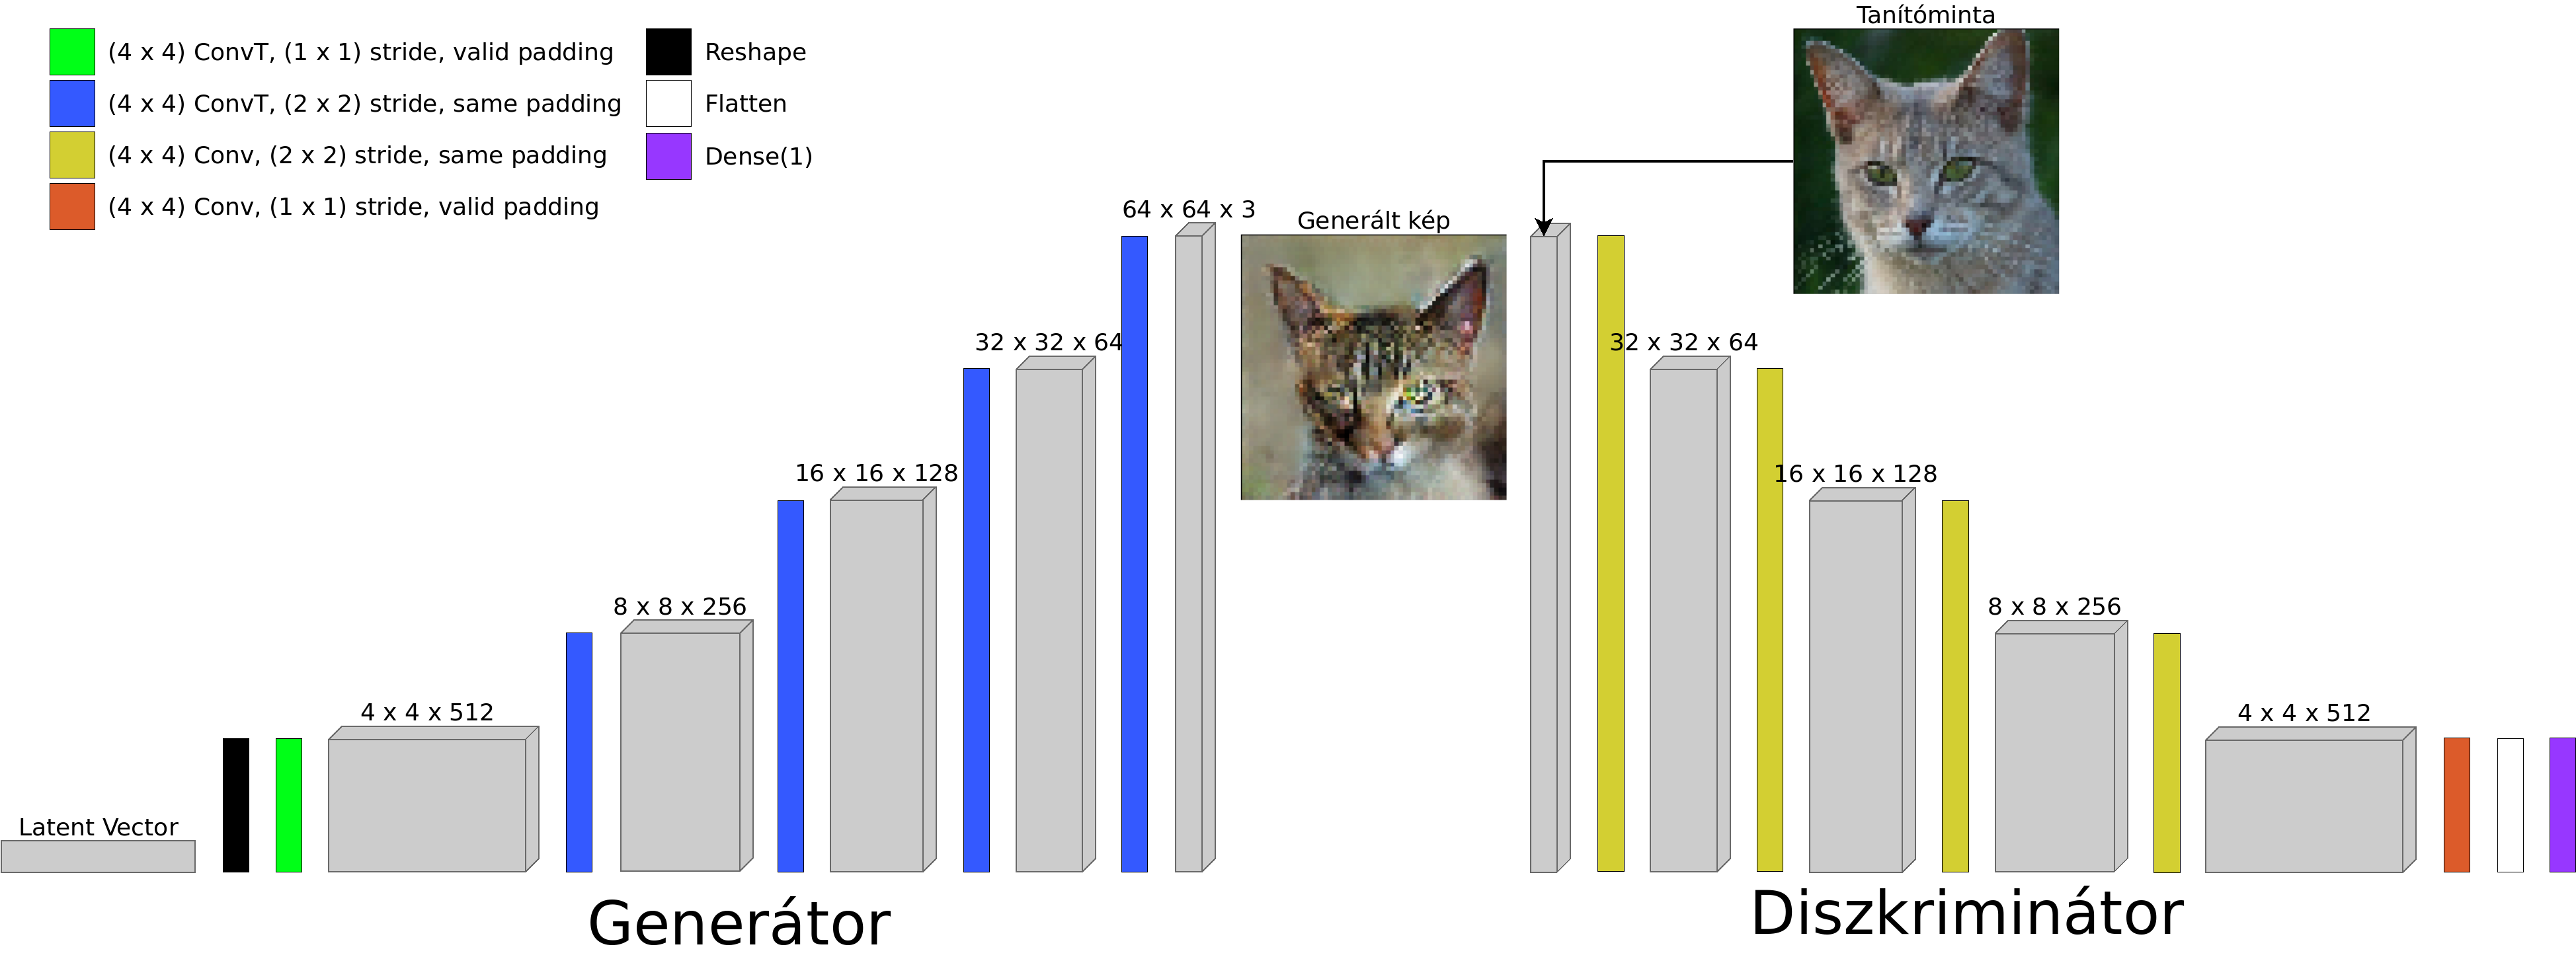
\includegraphics[width=15cm]{images/DCGAN.png}
\caption{DCGAN architektúra}
\label{fig:dcgan}
\end{figure}

\SubSection{Generátor}

Az osztályozáshoz használt konvolúciós hálókkal ellentétben a Generátorban a kisebb felbontás felől haladunk a nagyobb felbontásig.
A generátor modellem első implementációjában \textit{Dekonvolúciós} rétegeket alkalmaztam, amelyet \textit{Transzponált konvolúciós} rétegnek is nevezhetünk. A dekonvolúció a konvolúció ellentettje, vagyis a feladata, hogy egy alacsonyabb dimenziójú reprezentációt magasabb dimenzióba emeljen. Segítségével minden rejtett réteg kimenete egy nagyobb felbontású kép lesz. Tehát a hálónak jelen esetben meg kell tanulnia a rétegekben az optimális felbontás-növelést. Előre megadott paraméterek a filterek darabszáma, a kernel mérete, a strides(?) és a padding. Ha a padding-ot "same"-re és ha a strides paramétert $2 \times 2$-esnek választjuk, úgy a réteg kimenetén megjelenő kép felbontása kétszerese lesz a bemeneti oldalon megfigyelhető képnek. A rejtett rétegekben kezdetben ReLU aktivációs függvényt használtam, a neuronok kezdő értékeit a He inicializációs technikával \cite{he2015delving} állítottam be.

\begin{figure}[h]
\centering
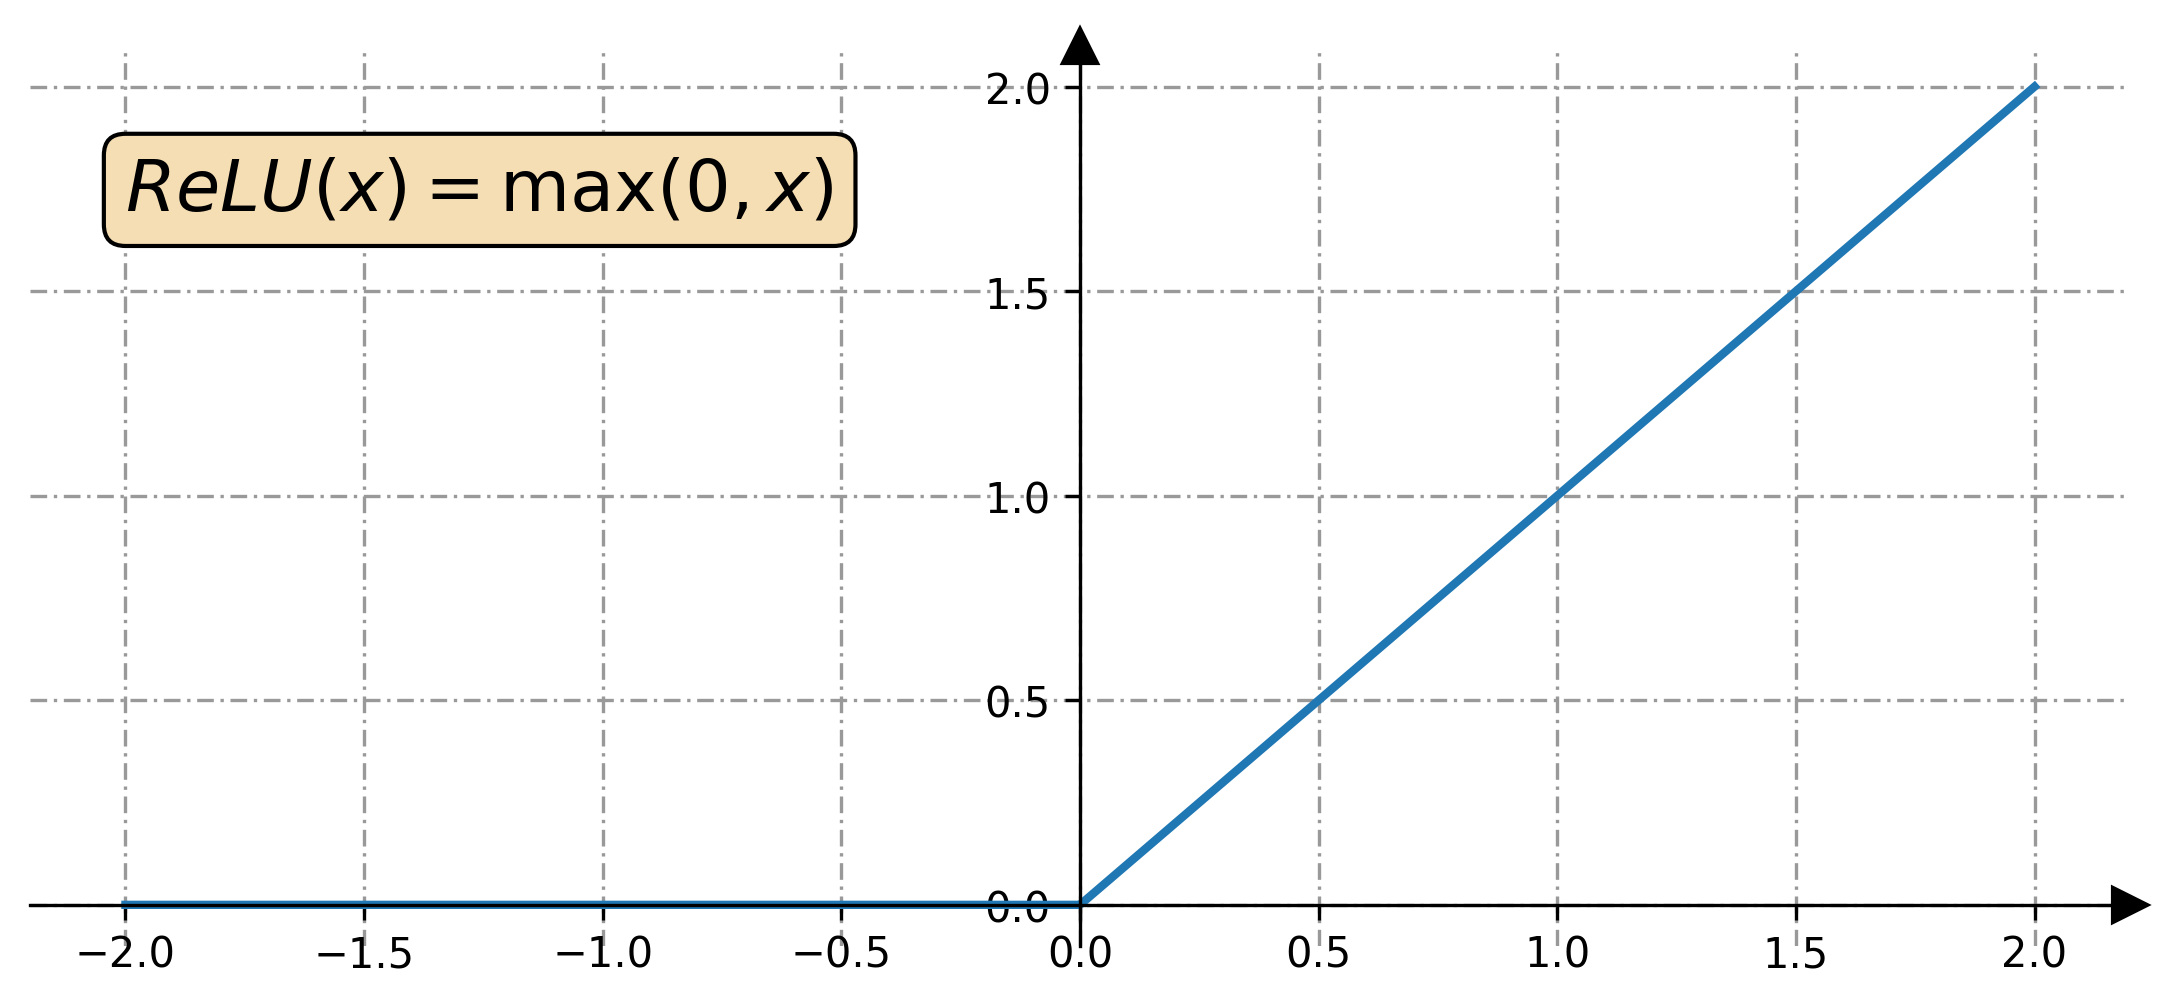
\includegraphics[width=10cm]{images/relu.png}
\caption{ReLU aktivációs függvény}
\label{fig:relu}
\end{figure}

A tanításhoz célszerű a kép pixeleinek intenzitását normalizálni a $[-1, 1]$ intervallumra lebegőpontos értékekre. A Generátor is ebben az intervallumban fogja a képek pixeleit generálni a hiperbolikus tangens kimeneti aktivációs függvényéből adódóan. (tanh indoklás, sigmoid helyett..) A megjelenítéshez később természetesen denormalizálnunk kell a generált képek pixelértékeit a $[0, 255]$ tartományra.

A Generátor modell bemenetként az előre definiált látens tér dimenziójával megegyező dimenziójú zajt kap, vagyis annak a $z_n$ dimenziószámú térnek egy pontját. Majd ezen bemeneti zaj segítségével állítja össze a megfelelő kimeneti képet. A tanulás során tehát a látens tér tartományaihoz rendeli a tanult jellegzetességeket és a látens teret mintavételezve dekódolható a Generátor segítségével a ponthoz tartozó kép.

A bemeneti zaj egy \textit{Reshape} rétegen megy keresztül, amelyben a látens tér dimenziószámát átformázza egy $1 \times 1 \times z_n$ dimenziójú mátrixszá. Ezen réteg kimenetével a későbbi dekonvolúciós rétegek már tudnak dolgozni.
Ezután az első dekonvolúciós rétegen megy át a kapott mátrix, amely 512 darab filtert tartalmaz, $4 \times 4$-es kernelméretekkel dolgozik és 'valid' paddingot használ. Az aktivációs függvénye ReLU a már említett He inicializálással. Ezen lépés arra szolgál, hogy a látens térből előállítson egy $4 \times 4 \times 512$ alakú tensort, amely az első, legkisebb felbontású képünknek tekinthetjük ebben az esetben, ahol a színcsatornák száma 512 és a felbontása pedig $4 \times 4$.

A Generátorban ezután $2 \times 2$-es stride értékeket használva same padding-gel a kívánt felbontásig dekonvolúciós rétegeken keresztül növekszik a felbontás. A kernelméretét a rétegekben egységesen $4 \times 4$-ra állítottam be. Az aktivációs függvény szintén ReLU. A rétegekben haladva a filterek darabszáma pedig feleződik. A filterek optimális számára csupán csak empirikus eredményeket találtam, így a paraméterek száma viszonylag alacsonyabban tartható és a tanítás ideje is lecsökken.

A kimeneti képnek olyan tulajdonságokkal kell rendelkeznie, mint a tanítómintában szeplő képeknek. Például ha a tanítóminta színes képekből áll, \textit{RGB} színkeveréssel, vagyis három színcsatornával, úgy a Generátor kimenetén is ilyen képekre van szükségünk. Mivel az említett dekonvolúciós rétegek több mint 3 színcsatornával dolgoztak, a megjeleníthetőség miatt szükséges tehát az utolsó dekonvolúciós rétegben a 3 darab filter, amely egyaránt transzponálja az előző réteg reprezentációit az egyel magasabb felbontás értékbe, és a csatornák számát pedig 3-ra állítja.
Egyes GAN architektúrákban ez az utolsó réteg csupán a 3 színcsatornába vetítést végzi el konvolúciós réteggel és szokás \textit{to RGB} rétegnek is nevezni \cite{karras2017progressive, karras2019style, karnewar2020msg}. Viszont jelen esetben egyúttal a felbontást is növeli a példámban szereplő utolsó réteg, ha $1 \times 1$-es stride értékkel rendelkezne ez a dekonvolúciós réteg, akkor valójában úgy működne mint egy konvolúciós réteg és tényleg csak a csatornák számát változtatná meg. Viszont akkor szükség lenne még egy felbontásnövelő rétegre, amely tovább növelné a paraméterek számát.

Végül a hiperbolikus tangens aktivációs függvény hatására az eredményeket a $[-1, 1]$ intervallumba transzformálja.

Az alábbi kódrészletben látható a felvázolt generátor architektúra megvalósítása a keras \textit{Sequential API}-ja segítségével.

\begin{python}
generator = keras.Sequential([
    keras.layers.Reshape((1, 1, 100), input_shape=[100]),
    keras.layers.Conv2DTranspose(512, (4, 4), (1, 1), 'valid',
                                 activation="relu",
                                 kernel_initializer="he_normal"),
    keras.layers.Conv2DTranspose(256, (4, 4), (2, 2), 'same',
                                 activation="relu",
                                 kernel_initializer="he_normal"),
    keras.layers.Conv2DTranspose(128, (4, 4), (2, 2), 'same',
                                 activation="relu",
                                 kernel_initializer="he_normal"),
    keras.layers.Conv2DTranspose(64, (4, 4), (2, 2), 'same',
                                 activation="relu",
                                 kernel_initializer="he_normal"),
    keras.layers.Conv2DTranspose(3, (4, 4), (2, 2), 'same',
                                 activation="relu"),
    keras.layers.Activation("tanh")
])
\end{python}

\begin{figure}[h]
\centering
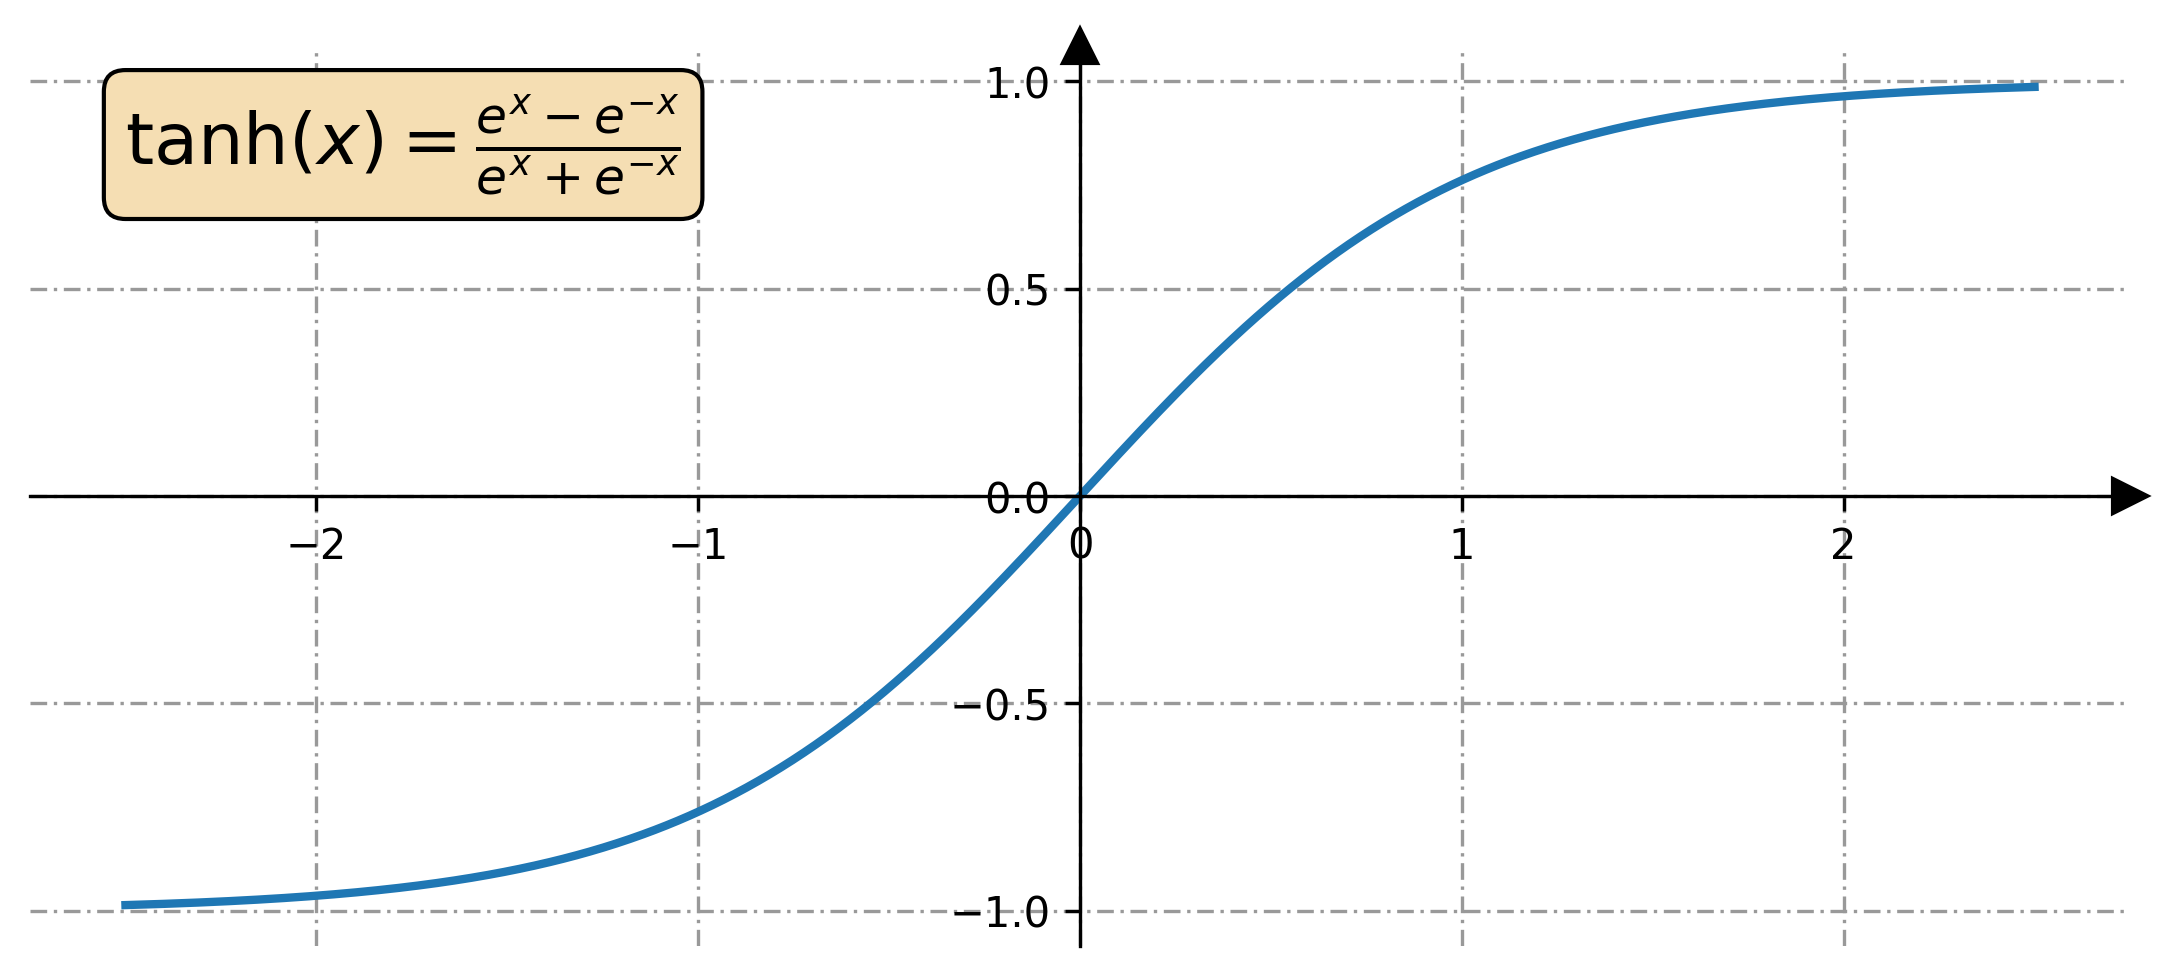
\includegraphics[width=10cm]{images/tanh.png}
\caption{Hiperbolikus tangens aktivációs függvény}
\label{fig:tanh}
\end{figure}

\SubSection{Diszkriminátor}

A Diszkriminátor modell lényegében egy bináris osztályozó, amely eldönti, hogy a bemenetül kapott kép valódi-e vagy hamis. A bemeneti kép konvolúciós rétegeken megy végig, kinyerve a jellegzetességeket és felállítva egy olyan belső reprezentációt, amely alapján az utolsó \textit{dense} réteg megfelelő kimenettel tud rendelkezni. A képen található mintázatokat a konvolúciós rétegek filterek segítségével tanulja meg, amelyek megadott kernelméretekben pásztázzák végig a bemenetet. Így az egyes konvolúciós rétegek kimeneteként egy olyan reprezentáció jön létre a bemeneti képről, amelyben érvényesülnek a pixeleket körülölelő további pixelek kapcsolatai is. Ezáltal az utolsó előtti réteg, a szerializáció (\textit{Flattening}) kevésbé fogja a kép tartalmára vonatkozó információt rontani. Mivel a tanítóminta képeinek pixelértékeit normalizáltuk a $[-1, 1]$ intervallumra, így a diszkriminátor a bemenetén is ilyen tulajdonságú képeket vár. A Diszkriminátor felépítésben hasonlít a Generátorhoz, lényegében annak tükörképeként képzelhetjük el. Viszont a dekonvolúciós rétegek helyett konvolúciós rétegeket alkalmazunk benne a jellegzetességek kinyerésére. Majd ha eljutunk a kívánt dimenziószámig, egy teljesen összekötött rétegben hozza meg a modell a döntést.

A generátorhoz hasonlóan az alábbi kódrészlet bemutatja a felvázolt diszkriminátor keras Sequential API-val történő megvalósítását:
\begin{python}
discriminator = keras.Sequential([
    keras.layers.Conv2D(64, (4, 4), (2, 2), "same",
                        input_shape=(64, 64, 3), activation="relu",
                        kernel_initializer="he_normal"),
    keras.layers.Conv2D(128, (4, 4), (2, 2), "same", activation="relu",
                        kernel_initializer="he_normal"),
    keras.layers.Conv2D(256, (4, 4), (2, 2), "same", activation="relu",
                        kernel_initializer="he_normal"),
    keras.layers.Conv2D(512, (4, 4), (2, 2), "same", activation="relu",
                        kernel_initializer="he_normal"),
    keras.layers.Conv2D(100, (4, 4), (1, 1), "valid", activation="relu"),
    keras.layers.Flatten(),
    keras.layers.Dense(1)
])
\end{python}

Mint a kódrészletből is látható, az utolsó teljesen összekötött rétegnek nincsen aktivációs függvénye. A sigmoid függvényt a keresztentrópia számolásnál alkalmazzuk majd a dense réteg kimenetére, amely megkönnyíti a tanítást. (??)

Az alábbi táblázatokban összefoglalom az architektúra felépítését:
\begin{center}

\begin{tabular}{c c}

\scriptsize{
\begin{tabular}{ |p{1.7cm}|p{1.5cm}|p{1.6cm}| }
	\hline
	\multicolumn{3}{|c|}{\textbf{Generátor}} \\
	\hline
	Réteg & Aktivációs függvény & Kiement alakja\\
	\hline
	Input & - & (100)\\
	Reshape & - & (1, 1, 100)\\
	(4x4) ConvT & ReLU & (4, 4, 512)\\
	(4x4) ConvT & ReLU & (8, 8, 256)\\
	(4x4) ConvT & ReLU & (16, 16, 128)\\
	(4x4) ConvT & ReLU & (32, 32, 64)\\
	(4x4) ConvT & tanh & (64, 64, 3)\\
	\hline
	\multicolumn{3}{|r|}{Paraméterek száma: \textbf{3.5 millió}} \\
	\hline
\end{tabular}}

&\scriptsize{
\begin{tabular}{ |p{1.7cm}|p{1.5cm}|p{1.6cm}| }
	\hline
	\multicolumn{3}{|c|}{\textbf{Diszkriminátor}} \\
	\hline
	Réteg & Aktivációs függvény & Kiement alakja\\
	\hline
	Input & - & (64, 64, 3)\\
	(4x4)Conv & ReLU & (32, 32, 64)\\
	(4x4)Conv & ReLU & (16, 16, 128)\\
	(4x4)Conv & ReLU & (8, 8, 256)\\
	(4x4)Conv & ReLU & (4, 4, 512)\\
	(4x4)Conv & ReLU & (1, 1, 100)\\
	Flatten & - & (100)\\
	Dense(1) & - & (1)\\
	\hline
	\multicolumn{3}{|r|}{Paraméterek száma: \textbf{3.5 millió}} \\
	\hline
\end{tabular}}

\end{tabular}
\end{center}

\SubSection{Tanítás, mérések}

A felvázolt architektúrát az Adam optimalizációs módszerrel, 0.0004 \textit{learning rate} hiperparaméter mellett tanítva a hibaértékek a következő ábrához hasonlóan alakulnak:

\begin{figure}[h]
\centering
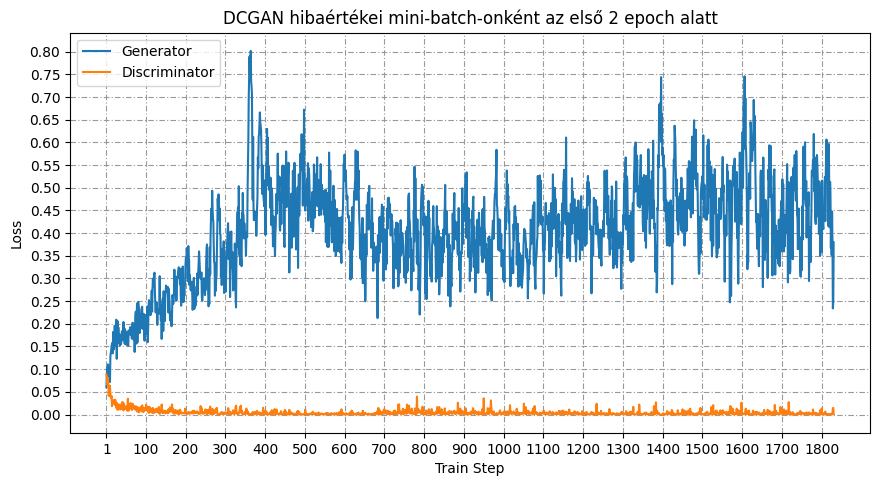
\includegraphics[width=15cm]{images/miniloss.png}
\caption{Hibaértékek mini-batch-onként}
\label{fig:mini-batch_loss_plot}
\end{figure}

Egy tanítási lépés egy mini-batch-on történő tanítást jelent, egy epoch pedig az összes mini-batch-on való tanítást jelenti.
Ha csak a nyers hibaértékre tekintünk, akkor azt figyelhetjük meg, hogy a tanítási lépések között erősen oszcillálnak az értékek. Kijelenthetjük a látott eredmények alapján, hogy a tanítás valóban nem stabil és látszólag egészen random módon változhatnak az értékek.
A szemléltetés kedvéért a következő ábrán a mini-batchokon számolt hibaértékek átlagait figyelhetjük meg epoch-onként.

\begin{figure}[h]
\centering
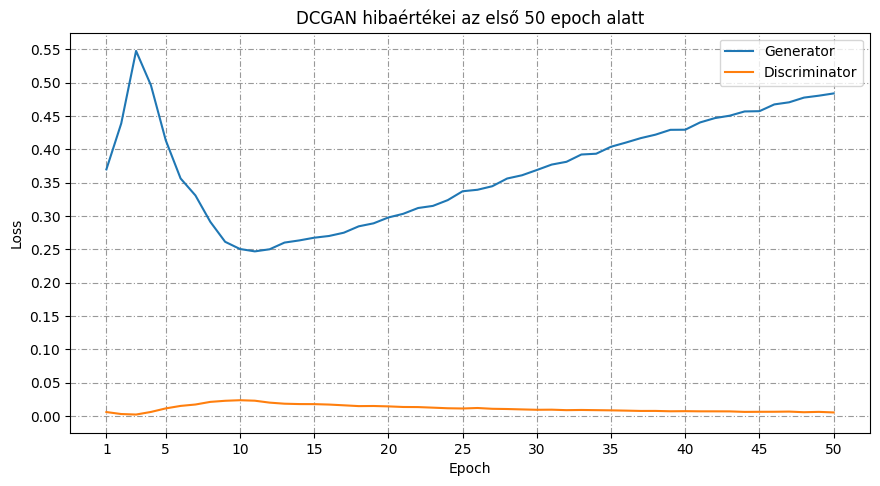
\includegraphics[width=15cm]{images/epochloss.png}
\caption{Hibaértékek epoch-onként}
\label{fig:epoch_loss_plot}
\end{figure}

Így finomabb görbéket kapunk, viszont erősen torzít az ábra, hiszen a GAN tanítási folyamata nem ilyen rendezett, mint ahogyan az első ábrán is láthattuk.
A hibaértékek változását vizsgálva megfigyelhető a versengés, vagyis hogy a két hálózat hibái mennyire ellentétesen mozognak az epoch-ok alatt. Mivel a tanulás során függőség van a két hálózat között, így ha a diszkriminátor egy vizsgált epoch alatt rosszabbul teljesítene a korábbi eredményekhez képest, akkor az a generátor javára válik és annak hibaértéke alacsonyabb lesz és fordítva. A generátor hibái többszörösek lehetnek a diszkriminátor hibáinak, de ez a jelenség teljesen természetes, hiszen a generátor lényegében a másik hálózat hibáiból tud csak tanulni, mivel a tanulás során nem látja a tanítóminta elemeit. A generátorban megfigyelhető, egyre növekvő hibaérték ellenére a generált képek minősége és részletezettsége is növekedni fog.

A hibaértékekből nem vonhatunk le pontos következtetéseket, így a fenti ábrák csupán szemléltetésképp készültek el. A GAN teljesítményének mérésére egyéb ajánlások jelentek meg, ilyen az Inception Score \cite{salimans2016improved} és az Fréchet Inception Distance \cite{heusel2017gans}.

\SubSection{Az architektúra gyengeségei, problémái}

A modell természetesen bővíthető tetszőlegesen nagy felbontásig, a felbontást növelő rétegek számával. Viszont az architektúrával problémák léphetnek fel:
\begin{itemize}
	\item A modell ebben a formájában igen hajlamos az mode collapse-re, vagyis a tanulás során jelentkező összeomlásra.
	\item A konvolúciós rétegek működéséből adódóan csupán lokális pixel-környezetekre képes összefüggő részeket generálni a modell.
	Ez a működés alacsony felbontás mellett is anomáliákat idézhet elő, ilyen a képeken megfigyelhető ismétlődő, sakkmintás zaj. Ha a rejtett konvolúciós rétegek számával növelnénk a felbontást, akkor további nehézségbe is ütközünk: a modell nem lesz képes felismerni és megtanulni a tanítóminta képein megfigyelhető távoli, összefüggő tulajdonságokat. Így a generált képek részletezettsége alacsony lesz, gyakran blobokat figyelhetünk meg csupán, különböző textúrákkal. A globális összefüggőségre több javaslat is érkezett a DCGAN megjelenése óta...
	\item A modellnek nincsen információja a különféle osztályokról, csupán a képek rendezetlen halmazán tanul, így magától kell megtanulnia a különféle osztályok jellegzetességeit.
	Az általánosítás szempontjából ez előnyös is lehet, viszont ha merőben különböző osztályokra szeretnénk betanítani a modellt, akkor az úgynevezett \textit{class conditoning} nélkül ezt igen nehezen tudnánk megvalósítani.
\end{itemize}

\SubSection{Sakkmintázat kiküszöbölése}

\begin{figure}[h]
\centering
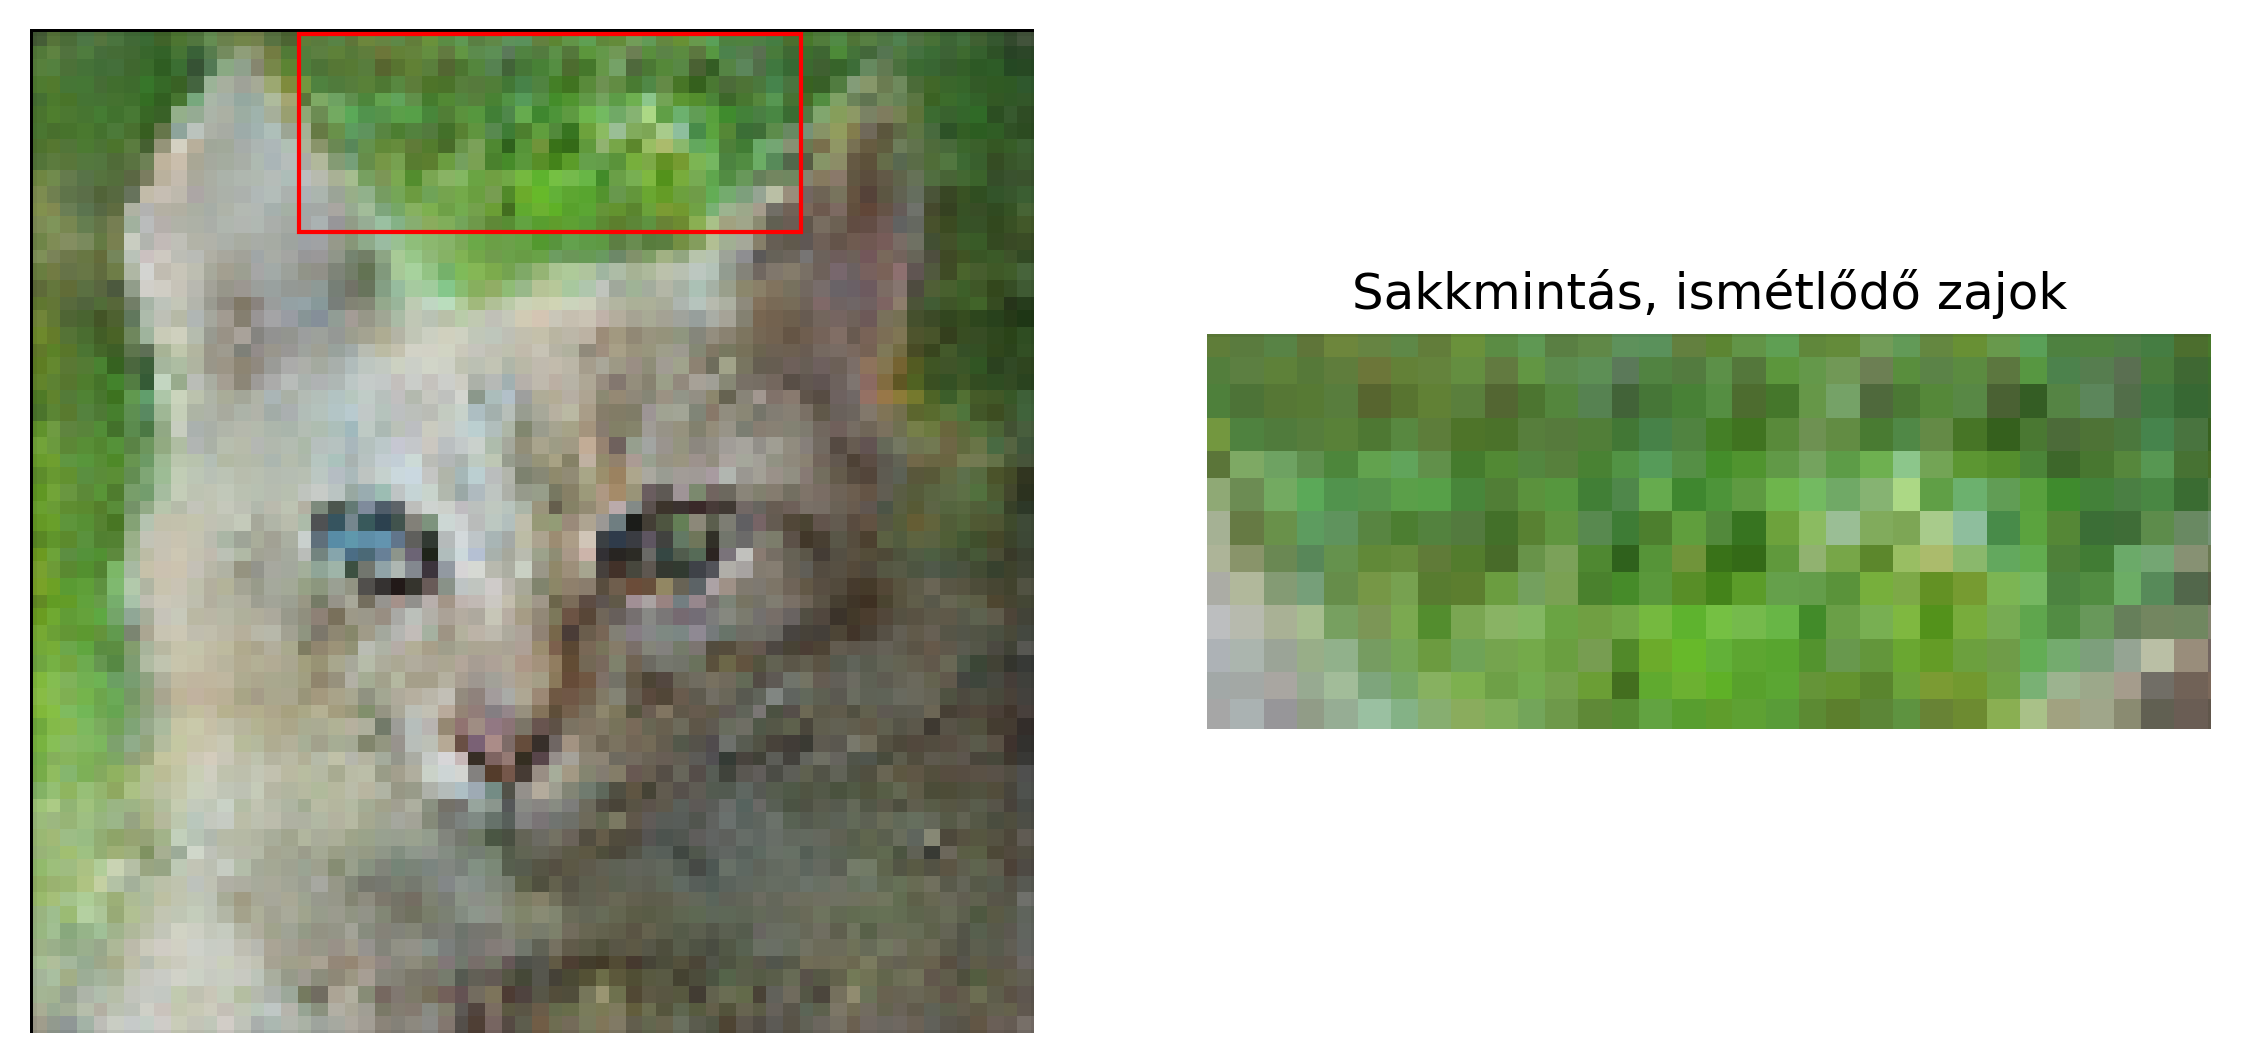
\includegraphics[width=13cm]{images/chessboard-patterns.png}
\caption{Jellegzetes zajok a generált képeken}
\label{fig:chessboard-patterns}
\end{figure}

https://distill.pub/2016/deconv-checkerboard/

A cikkben a Dekonvolúciós rétegek helyett a Konvolúciós és UpSampling rétegeket ajánlották bilineáris interpolációval. Vagyis a felbontásnövelési feladatot elvették a dekonvolúciós rétegtől és egy tanítható-paraméter nélküli rétegre bízták a feladatot, aminek csak annyi a szerepe, hogy a felbontást növelje. Ezzel az ötlettel a sakkmintás zajt igen jól leredukálták a generált képeken. A tanítás előtti Generátor kimenetén is megfigyelhető, hogy a kép "lágyabb", kevésbé rendezettebb, mint az előző példában.

Viszont így önmagában nem volt szerencsém a modellt tanulásra bírnom és a BatchNormalization regularizációs rétegeket kellett beékelnem a modellbe. A technikát és a további alkalmazott regularizációs eljárásokat egy másik fejezetben foglalom majd össze.

\begin{python}
def add_upsampling_unit(model,
                        filters, kernel_size):
    model.add(
        Conv2D(
            filters=filters,
            kernel_size=kernel_size,
            padding='same',
            activation="relu",
            kernel_initializer="he_normal"
        )
    )
    model.add(UpSampling2D())
\end{python}

\begin{figure}[h]
\centering
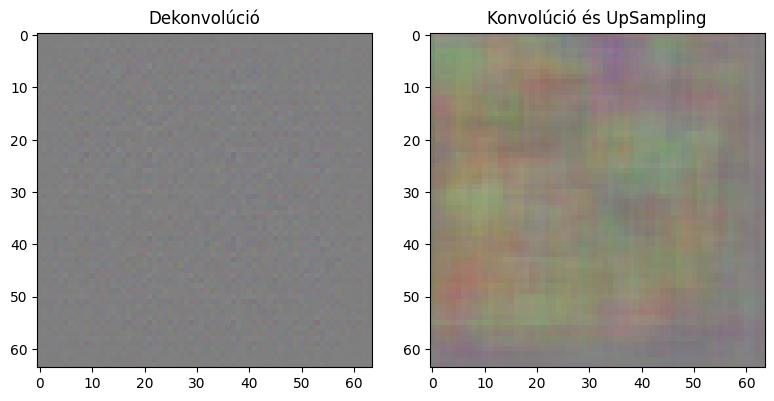
\includegraphics[width=13cm]{images/deconv-vs-conv_upsmpl.png}
\caption{Tanítás előtti Generátor kimenetei}
\label{fig:deconv-vs-conv_upsmpl}
\end{figure}